\section{Software Development Life Cycle}
\label{sec:sdlc}

...

\ac{SDLC}\index{software development life cycle}

In more technical side, the \ac{SDLC} of this software follows or tends to assist a software development principle called \ac{DRY}\index{don't repeat yourself},
which every piece of knowledge must have a single, unambiguous, authoritative representation within a system,~\autocite{Hunt1999Pragmatic}
That means the content that potentially will be duplicated must only in a single part and be reusable.
Therefore code then resulted in a cleaner and clearer structure.
This applied as well as in test plans, the build system, and documentation within or outside the code.
Also happens in the user interaction design, therefore there is a decreased amount of duplicated data that is accidentally created or not intended by users.

% --------------------------------------------------
\subsection{Agile Methodologies}

Agile is a time boxed, iterative approact to software delivery that builds software incrementally from the start of the project, instead of trying to deliver it all at once near the end.
It works by breaking projects down into little bits of user functionality called user stories, prioritizing them, and then continuously delivering them in short two week cycles called iterations.~\autocite{Rasmusson2015Agile}
Therefore, we don't risk in creating a big or even a thing that small for a long time.
Because we iterate the result, coming back again as like a beginning.
Essentially, we learn and relearn what we could have done in each iteration process.
In a process matter of sense, analysis, design, development/coding, and testing are continuous activities.
In addition, there are a lot of other aspects that required:

\begin{easylist}
& Development itself is iterative
& Planning is adaptive
& The scope variables may vary
& Requirements can change over time
& Working software is the primary measure of success
& and other leaned segments to consider
\end{easylist}

%TODO Agile illustration

% --------------------------------------------------
\subsection{Minimum Viable Product}

Agile methodologies also heavily corresponds with building a \ac{MVP}\index{Minimum Viable Product} or we can also called it a \ac{MWT}\index{Minimum Working Thing}. Shortly defined, each elements of \ac{MVP} are~\autocite{Montgomery2013MWT}:

\begin{description}
  \item[Minimum] The least or smallest amount possible.
  \item[Viable] Capable of working successfully.
  \item[Product] An article or substance that is created or refined for sale.
\end{description}

In conclusion, \ac{MVP} is a...
%TODO

\begin{figure}[htb]
    \centering
    \includegraphics[width=\textwidth]{\dir/include/mvp-1}
    \caption[MVP illustrated]{MVP illustrated with only one usable product and some incremental products~\autocite{Mercury2014MVP}}
    \label{fig:method:mvp-1}
\end{figure}

We can also illustrate it as creating a vehicle with two different steps.
As in \autoref{fig:method:mvp-1}, the first one is a need to take a lot of steps of before finally finished the final usable product.
The second one is an incremental steps of creating the usable product, until it's final yet to be usable as visioned and planned.
It can be seen that the second approach is more appealing and effective than the first.

\begin{figure}[htb]
    \centering
    \includegraphics[width=\textwidth]{\dir/include/mvp-2}
    \caption[MVP compared]{MVP compared with unusable and complete product~\autocite{Mercury2014MVP}}
    \label{fig:method:mvp-2}
\end{figure}

Also as in \autoref{fig:method:mvp-2}, \ac{MVP} is compared with unusable product and complete product.
In this context, \ac{MVP} is ideally more balanced and preferable than the others.
More than that, if there is more effort and time, we can build a \ac{MLP}\index{Minimum Loveable Product}.
Which is an \ac{MVP} but taken beyond a working thing, which the customer will actually love using.
It's an embodiment of a production ready and could potentially get a customer or lots of them.
The thing that matters and can be used well.
Although it expected to be a real matter, such preliminary model like a protoype, a mockup, or even a set of data can sometimes considered as an \ac{MVP}.

% --------------------------------------------------
\subsection{Business Model Canvas}

Because thesis procedure has a very limited time, we can only took the limit until it is viable enough yet basically usable.
We first only focus on the main basic features.
Yet, the development will always be continued further as a product of startup.
The code and supporting commpents themself will be released as an open source project.
So with the backing help of company and endorsement of community, this could handed by a lot of people.

But then, which \ac{MVP} that is most required to be used?
Since we're creating a software product for people, there is a concern to make it viable for business too.
We can determine that by using a business model tool called \ac{BMC}\index{Business Model Canvas}.
Related to \ac{MVP}, \ac{BMC} includes the most important components which are Customer Segments and Value Propositions.
Business Model Canvas is a strategic management and lean startup template for developing new or documenting existing business models.
It is a visual chart with elements describing a firm's value proposition, infrastructure, customers, and finances.
It assists firms in aligning their activities by illustrating potential trade-offs.
% TODO

So with the Business Model Canvas, we can map out your entire business model in one image.
This works for startup entrepreneurs, just as well as for the most senior executives.~\autocite{Strategyzer2011BMC}
\autoref{fig:bmc:blank} shows how the blank Business Model Canvas looks like.

\begin{figure}[htbp]
    \centering
    %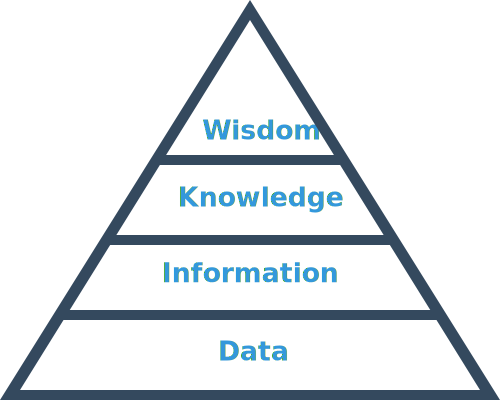
\includegraphics[width=4cm]{\dir/include/dikw-pyramid.png}
    \caption{Business Model Canvas}
    \label{fig:bmc:blank}
\end{figure}

For each building blocks...
%TODO

% --------------------------------------------------
\subsection{Extreme Programming}

Since

%TODO illustration
%TODO Reason
%TODO About documentation

% --------------------------------------------------
\subsection{Scrum and Kanban}

...
Other

%TODO Reason
%TODO About documentation

% --------------------------------------------------
\subsection{Testing with NAME}

Because...

%TODO Reason
